\section{Applying HDM on BraTS}
\nblink{23\_brats\_hdm\_per\_modality-circle10.ipynb}
\nblink{23\_brats\_hdm\_per\_modality-circle15.ipynb}
\nblink{23\_brats\_hdm\_per\_modality-circle20.ipynb}
\nblink{23\_brats\_hdm\_per\_modality-circle25.ipynb}

Once per image
Per modality would probably produce better results.

\subsection{Scan Brats18\_TCIA02\_491\_1 layer 2}
\subsubsection{Results}


\begin{figure}[H]
    \centering
    \begin{subfigure}{.24\textwidth}
        \centering
        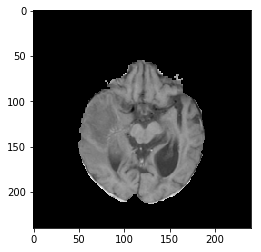
\includegraphics[width=\linewidth]{chapters/06_hdm/Brats18_TCIA02_491_1_L2/1.png}
        \caption{T1 modality slice}
    \end{subfigure}%
    \begin{subfigure}{.24\textwidth}
        \centering
        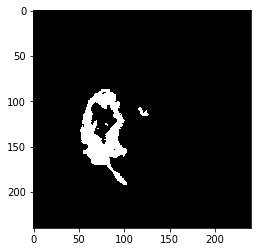
\includegraphics[width=\linewidth]{chapters/06_hdm/Brats18_TCIA02_491_1_L2/0.png}
        \caption{T1 modality ground truth tumor}
    \end{subfigure}
    \begin{subfigure}{.24\textwidth}
        \centering
        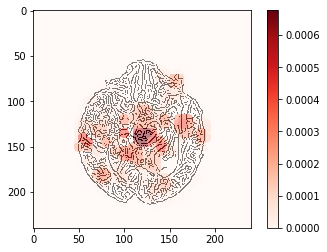
\includegraphics[width=\linewidth]{chapters/06_hdm/Brats18_TCIA02_491_1_L2/3.png}
        \caption{T1 modality with a third mask applied}
    \end{subfigure}
    \begin{subfigure}{.24\textwidth}
        \centering
        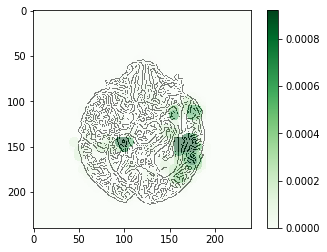
\includegraphics[width=\linewidth]{chapters/06_hdm/Brats18_TCIA02_491_1_L2/4.png}
        \caption{T1 modality with a third mask applied}
    \end{subfigure}
    \caption{Modality T1}
\end{figure}

\subsubsection{Discussion}

\subsection{Scan Brats18\_TCIA08\_242\_1 layer 2}

\subsubsection{Results}

\subsubsection{Discussion}

\subsection{Scan Brats18\_2013\_17\_1 layer 1}
\subsubsection{Results}

\subsubsection{Discussion}

\subsubsection{Conclusion}
it works!